\documentclass[oneside,final,14pt]{extreport}
%\documentclass[oneside,final,14pt]{extreport}
\usepackage[tmargin=2cm,rmargin=1in,lmargin=1in,margin=0.85in,bmargin=2cm,footskip=.2in]{geometry}
\usepackage[utf8]{inputenc}
\usepackage[T2A]{fontenc}
\usepackage[russianb]{babel}
\usepackage{amsmath,amsfonts,amsthm,amssymb,mathtools}
\usepackage{anyfontsize}
\usepackage[varbb]{newpxmath}
\usepackage{xfrac}
\usepackage{float}
\usepackage[makeroom]{cancel}
\usepackage{mathtools}
\usepackage{bookmark}
\usepackage{enumitem}
\usepackage{hyperref,theoremref}
\hypersetup{
  pdftitle={Assignment},
  colorlinks=true, linkcolor=doc!90,
  bookmarksnumbered=true,
  bookmarksopen=true
}
\usepackage[most,many,breakable]{tcolorbox}
\usepackage{xcolor}
\usepackage{varwidth}
\usepackage{etoolbox}
%\usepackage{authblk}
\usepackage{nameref}
\usepackage{multicol,array}
\usepackage{tikz-cd}
% \usepackage[ruled,vlined,linesnumbered]{algorithm2e}
\usepackage{comment} % enables the use of multi-line comments (\ifx \fi) 
\usepackage{import}
\usepackage{xifthen}
\usepackage{pdfpages}
\usepackage{transparent}
\graphicspath{{images/}}
\DeclareGraphicsExtensions{.pdf,.png,.jpg} 
\usepackage{algpseudocode}
\usepackage{algorithm}
\usepackage[linguistics]{forest}

% \newcommand\mycommfont[1]{\footnotesize\ttfamily\textcolor{blue}{#1}}
% \SetCommentSty{mycommfont}
% \newcommand{\incfig}[1]{%
%     \def\svgwidth{\columnwidth}
%     \import{./figures/}{#1.pdf_tex}
% }

\usepackage{tikzsymbols}
\renewcommand\qedsymbol{$\Laughey$}


%%%%%%%%%%%%%%%%%%%%%%%%%%%%%%
% SELF MADE COLORS
%%%%%%%%%%%%%%%%%%%%%%%%%%%%%%



\definecolor{myg}{RGB}{56, 140, 70}
\definecolor{myb}{RGB}{45, 111, 177}
\definecolor{myr}{RGB}{199, 68, 64}
\definecolor{mytheorembg}{HTML}{F2F2F9}
\definecolor{mytheoremfr}{HTML}{00007B}
\definecolor{mylenmabg}{HTML}{FFFAF8}
\definecolor{mylenmafr}{HTML}{983b0f}
\definecolor{mypropbg}{HTML}{f2fbfc}
\definecolor{mypropfr}{HTML}{191971}
\definecolor{myexamplebg}{HTML}{F2FBF8}
\definecolor{myexamplefr}{HTML}{88D6D1}
\definecolor{myexampleti}{HTML}{2A7F7F}
\definecolor{mydefinitbg}{HTML}{E5E5FF}
\definecolor{mydefinitfr}{HTML}{3F3FA3}
\definecolor{notesgreen}{RGB}{0,162,0}
\definecolor{myp}{RGB}{197, 92, 212}
\definecolor{mygr}{HTML}{2C3338}
\definecolor{myred}{RGB}{127,0,0}
\definecolor{myyellow}{RGB}{169,121,69}
\definecolor{myexercisebg}{HTML}{F2FBF8}
\definecolor{myexercisefg}{HTML}{88D6D1}


%%%%%%%%%%%%%%%%%%%%%%%%%%%%
% TCOLORBOX SETUPS
%%%%%%%%%%%%%%%%%%%%%%%%%%%%

\setlength{\parindent}{1cm}
%================================
% THEOREM BOX
%================================

\tcbuselibrary{theorems,skins,hooks}
\newtcbtheorem[number within=section]{Theorem}{Теорема}
{%
  enhanced,
  breakable,
  colback = mytheorembg,
  frame hidden,
  boxrule = 0sp,
  borderline west = {2pt}{0pt}{mytheoremfr},
  sharp corners,
  detach title,
  before upper = \tcbtitle\par\smallskip,
  coltitle = mytheoremfr,
  fonttitle = \bfseries\sffamily,
  description font = \mdseries,
  separator sign none,
  segmentation style={solid, mytheoremfr},
}
{th}

\tcbuselibrary{theorems,skins,hooks}
\newtcbtheorem[number within=chapter]{theorem}{Теорема}
{%
  enhanced,
  breakable,
  colback = mytheorembg,
  frame hidden,
  boxrule = 0sp,
  borderline west = {2pt}{0pt}{mytheoremfr},
  sharp corners,
  detach title,
  before upper = \tcbtitle\par\smallskip,
  coltitle = mytheoremfr,
  fonttitle = \bfseries\sffamily,
  description font = \mdseries,
  separator sign none,
  segmentation style={solid, mytheoremfr},
}
{th}

\tcbuselibrary{theorems,skins,hooks}
\newtcolorbox{Theoremcon}
{%
  enhanced
  ,breakable
  ,colback = mytheorembg
  ,frame hidden
  ,boxrule = 0sp
  ,borderline west = {2pt}{0pt}{mytheoremfr}
  ,sharp corners
  ,description font = \mdseries
  ,separator sign none
}

%================================
% Corollary
%================================
\tcbuselibrary{theorems,skins,hooks}
\newtcbtheorem[number within=section]{Corollary}{Следствие}
{%
  enhanced
  ,breakable
  ,colback = myp!10
  ,frame hidden
  ,boxrule = 0sp
  ,borderline west = {2pt}{0pt}{myp!85!black}
  ,sharp corners
  ,detach title
  ,before upper = \tcbtitle\par\smallskip
  ,coltitle = myp!85!black
  ,fonttitle = \bfseries\sffamily
  ,description font = \mdseries
  ,separator sign none
  ,segmentation style={solid, myp!85!black}
}
{th}
\tcbuselibrary{theorems,skins,hooks}
\newtcbtheorem[number within=chapter]{corollary}{Следствие}
{%
  enhanced
  ,breakable
  ,colback = myp!10
  ,frame hidden
  ,boxrule = 0sp
  ,borderline west = {2pt}{0pt}{myp!85!black}
  ,sharp corners
  ,detach title
  ,before upper = \tcbtitle\par\smallskip
  ,coltitle = myp!85!black
  ,fonttitle = \bfseries\sffamily
  ,description font = \mdseries
  ,separator sign none
  ,segmentation style={solid, myp!85!black}
}
{th}

%================================
% LENMA
%================================

\tcbuselibrary{theorems,skins,hooks}
\newtcbtheorem[number within=section]{Lenma}{Лемма}
{%
  enhanced,
  breakable,
  colback = mylenmabg,
  frame hidden,
  boxrule = 0sp,
  borderline west = {2pt}{0pt}{mylenmafr},
  sharp corners,
  detach title,
  before upper = \tcbtitle\par\smallskip,
  coltitle = mylenmafr,
  fonttitle = \bfseries\sffamily,
  description font = \mdseries,
  separator sign none,
  segmentation style={solid, mylenmafr},
}
{th}

\tcbuselibrary{theorems,skins,hooks}
\newtcbtheorem[number within=chapter]{lenma}{Лемма}
{%
  enhanced,
  breakable,
  colback = mylenmabg,
  frame hidden,
  boxrule = 0sp,
  borderline west = {2pt}{0pt}{mylenmafr},
  sharp corners,
  detach title,
  before upper = \tcbtitle\par\smallskip,
  coltitle = mylenmafr,
  fonttitle = \bfseries\sffamily,
  description font = \mdseries,
  separator sign none,
  segmentation style={solid, mylenmafr},
}
{th}

%================================
% PROPOSITION
%================================

\tcbuselibrary{theorems,skins,hooks}
\newtcbtheorem[number within=section]{Prop}{Предложение}
{%
  enhanced,
  breakable,
  colback = mypropbg,
  frame hidden,
  boxrule = 0sp,
  borderline west = {2pt}{0pt}{mypropfr},
  sharp corners,
  detach title,
  before upper = \tcbtitle\par\smallskip,
  coltitle = mypropfr,
  fonttitle = \bfseries\sffamily,
  description font = \mdseries,
  separator sign none,
  segmentation style={solid, mypropfr},
}
{th}

\tcbuselibrary{theorems,skins,hooks}
\newtcbtheorem[number within=chapter]{prop}{Предложение}
{%
  enhanced,
  breakable,
  colback = mypropbg,
  frame hidden,
  boxrule = 0sp,
  borderline west = {2pt}{0pt}{mypropfr},
  sharp corners,
  detach title,
  before upper = \tcbtitle\par\smallskip,
  coltitle = mypropfr,
  fonttitle = \bfseries\sffamily,
  description font = \mdseries,
  separator sign none,
  segmentation style={solid, mypropfr},
}
{th}

%================================
% CLAIM
%================================

\tcbuselibrary{theorems,skins,hooks}
\newtcbtheorem[number within=section]{claim}{Утверждение}
{%
  enhanced
  ,breakable
  ,colback = myg!10
  ,frame hidden
  ,boxrule = 0sp
  ,borderline west = {2pt}{0pt}{myg}
  ,sharp corners
  ,detach title
  ,before upper = \tcbtitle\par\smallskip
  ,coltitle = myg!85!black
  ,fonttitle = \bfseries\sffamily
  ,description font = \mdseries
  ,separator sign none
  ,segmentation style={solid, myg!85!black}
}
{th}



%================================
% Exercise
%================================

\tcbuselibrary{theorems,skins,hooks}
\newtcbtheorem[number within=section]{Exercise}{Упражнение}
{%
  enhanced,
  breakable,
  colback = myexercisebg,
  frame hidden,
  boxrule = 0sp,
  borderline west = {2pt}{0pt}{myexercisefg},
  sharp corners,
  detach title,
  before upper = \tcbtitle\par\smallskip,
  coltitle = myexercisefg,
  fonttitle = \bfseries\sffamily,
  description font = \mdseries,
  separator sign none,
  segmentation style={solid, myexercisefg},
}
{th}

\tcbuselibrary{theorems,skins,hooks}
\newtcbtheorem[number within=chapter]{exercise}{Упражнение}
{%
  enhanced,
  breakable,
  colback = myexercisebg,
  frame hidden,
  boxrule = 0sp,
  borderline west = {2pt}{0pt}{myexercisefg},
  sharp corners,
  detach title,
  before upper = \tcbtitle\par\smallskip,
  coltitle = myexercisefg,
  fonttitle = \bfseries\sffamily,
  description font = \mdseries,
  separator sign none,
  segmentation style={solid, myexercisefg},
}
{th}

%================================
% EXAMPLE BOX
%================================

\newtcbtheorem[number within=section]{Example}{Пример}
{%
  colback = myexamplebg
  ,breakable
  ,colframe = myexamplefr
  ,coltitle = myexampleti
  ,boxrule = 1pt
  ,sharp corners
  ,detach title
  ,before upper=\tcbtitle\par\smallskip
  ,fonttitle = \bfseries
  ,description font = \mdseries
  ,separator sign none
  ,description delimiters parenthesis
}
{ex}

\newtcbtheorem[number within=chapter]{example}{Пример}
{%
  colback = myexamplebg
  ,breakable
  ,colframe = myexamplefr
  ,coltitle = myexampleti
  ,boxrule = 1pt
  ,sharp corners
  ,detach title
  ,before upper=\tcbtitle\par\smallskip
  ,fonttitle = \bfseries
  ,description font = \mdseries
  ,separator sign none
  ,description delimiters parenthesis
}
{ex}

%================================
% DEFINITION BOX
%================================

\newtcbtheorem[number within=section]{Definition}{Определение}{enhanced,
  before skip=2mm,after skip=2mm, colback=olive!5,colframe=olive!80!black,boxrule=0.5mm,
  attach boxed title to top left={xshift=1cm,yshift*=1mm-\tcboxedtitleheight}, varwidth boxed title*=-3cm,
  boxed title style={frame code={
          \path[fill=olive]
          ([yshift=-1mm,xshift=-1mm]frame.north west)
          arc[start angle=0,end angle=180,radius=1mm]
          ([yshift=-1mm,xshift=1mm]frame.north east)
          arc[start angle=180,end angle=0,radius=1mm];
          \path[left color=olive!60!black,right color=olive!60!black,
            middle color=olive!80!black]
          ([xshift=-2mm]frame.north west) -- ([xshift=2mm]frame.north east)
          [rounded corners=1mm]-- ([xshift=1mm,yshift=-1mm]frame.north east)
          -- (frame.south east) -- (frame.south west)
          -- ([xshift=-1mm,yshift=-1mm]frame.north west)
          [sharp corners]-- cycle;
        },interior engine=empty,
    },
  fonttitle=\bfseries,
  title={#2},#1}{def}

\newtcbtheorem[number within=chapter]{definition}{Определение}{enhanced,
  before skip=2mm,after skip=2mm, colback=olive!5,colframe=olive!80!black,boxrule=0.5mm,
  attach boxed title to top left={xshift=1cm,yshift*=1mm-\tcboxedtitleheight}, varwidth boxed title*=-3cm,
  boxed title style={frame code={
          \path[fill=olive]
          ([yshift=-1mm,xshift=-1mm]frame.north west)
          arc[start angle=0,end angle=180,radius=1mm]
          ([yshift=-1mm,xshift=1mm]frame.north east)
          arc[start angle=180,end angle=0,radius=1mm];
          \path[left color=olive!60!black,right color=olive!60!black,
            middle color=olive!80!black]
          ([xshift=-2mm]frame.north west) -- ([xshift=2mm]frame.north east)
          [rounded corners=1mm]-- ([xshift=1mm,yshift=-1mm]frame.north east)
          -- (frame.south east) -- (frame.south west)
          -- ([xshift=-1mm,yshift=-1mm]frame.north west)
          [sharp corners]-- cycle;
        },interior engine=empty,
    },
  fonttitle=\bfseries,
  title={#2},#1}{def}

%================================
% Solution BOX
%================================

\makeatletter
\newtcbtheorem{question}{Вопрос}{enhanced,
  breakable,
  colback=white,
  colframe=myb!80!black,
  attach boxed title to top left={yshift*=-\tcboxedtitleheight},
  fonttitle=\bfseries,
  title={#2},
  boxed title size=title,
  boxed title style={%
      sharp corners,
      rounded corners=northwest,
      colback=tcbcolframe,
      boxrule=0pt,
    },
  underlay boxed title={%
      \path[fill=tcbcolframe] (title.south west)--(title.south east)
      to[out=0, in=180] ([xshift=5mm]title.east)--
      (title.center-|frame.east)
      [rounded corners=\kvtcb@arc] |-
      (frame.north) -| cycle;
    },
  #1
}{def}
\makeatother

%================================
% SOLUTION BOX
%================================

\makeatletter
\newtcolorbox{solution}{enhanced,
  breakable,
  colback=white,
  colframe=myg!80!black,
  attach boxed title to top left={yshift*=-\tcboxedtitleheight},
  title=Solution,
  boxed title size=title,
  boxed title style={%
      sharp corners,
      rounded corners=northwest,
      colback=tcbcolframe,
      boxrule=0pt,
    },
  underlay boxed title={%
      \path[fill=tcbcolframe] (title.south west)--(title.south east)
      to[out=0, in=180] ([xshift=5mm]title.east)--
      (title.center-|frame.east)
      [rounded corners=\kvtcb@arc] |-
      (frame.north) -| cycle;
    },
}

%================================
% Question BOX
%================================

\makeatletter
\newtcbtheorem{qstion}{Вопрос}{enhanced,
  breakable,
  colback=white,
  colframe=mygr,
  attach boxed title to top left={yshift*=-\tcboxedtitleheight},
  fonttitle=\bfseries,
  title={#2},
  boxed title size=title,
  boxed title style={%
      sharp corners,
      rounded corners=northwest,
      colback=tcbcolframe,
      boxrule=0pt,
    },
  underlay boxed title={%
      \path[fill=tcbcolframe] (title.south west)--(title.south east)
      to[out=0, in=180] ([xshift=5mm]title.east)--
      (title.center-|frame.east)
      [rounded corners=\kvtcb@arc] |-
      (frame.north) -| cycle;
    },
  #1
}{def}
\makeatother

\newtcbtheorem[number within=chapter]{wconc}{Wrong Concept}{
  breakable,
  enhanced,
  colback=white,
  colframe=myr,
  arc=0pt,
  outer arc=0pt,
  fonttitle=\bfseries\sffamily\large,
  colbacktitle=myr,
  attach boxed title to top left={},
  boxed title style={
      enhanced,
      skin=enhancedfirst jigsaw,
      arc=3pt,
      bottom=0pt,
      interior style={fill=myr}
    },
  #1
}{def}
\makeatother

%================================
% NOTE BOX
%================================

\usetikzlibrary{arrows,calc,shadows.blur}
\tcbuselibrary{skins}
\newtcolorbox{note}[1][]{%
  enhanced jigsaw,
  colback=gray!20!white,%
  colframe=gray!80!black,
  size=small,
  boxrule=1pt,
  title=\textbf{Note:},
  halign title=flush center,
  coltitle=black,
  breakable,
  drop shadow=black!50!white,
  attach boxed title to top left={xshift=1cm,yshift=-\tcboxedtitleheight/2,yshifttext=-\tcboxedtitleheight/2},
  minipage boxed title=1.5cm,
  boxed title style={%
      colback=white,
      size=fbox,
      boxrule=1pt,
      boxsep=2pt,
      underlay={%
          \coordinate (dotA) at ($(interior.west) + (-0.5pt,0)$);
          \coordinate (dotB) at ($(interior.east) + (0.5pt,0)$);
          \begin{scope}
            \clip (interior.north west) rectangle ([xshift=3ex]interior.east);
            \filldraw [white, blur shadow={shadow opacity=60, shadow yshift=-.75ex}, rounded corners=2pt] (interior.north west) rectangle (interior.south east);
          \end{scope}
          \begin{scope}[gray!80!black]
            \fill (dotA) circle (2pt);
            \fill (dotB) circle (2pt);
          \end{scope}
        },
    },
  #1,
}

\newcommand{\thm}[2]{\begin{Theorem}{#1}{}#2\end{Theorem}}
\newcommand{\cor}[2]{\begin{Corollary}{#1}{}#2\end{Corollary}}
\newcommand{\mlenma}[2]{\begin{Lenma}{#1}{}#2\end{Lenma}}
\newcommand{\mprop}[2]{\begin{Prop}{#1}{}#2\end{Prop}}
\newcommand{\clm}[3]{\begin{claim}{#1}{#2}#3\end{claim}}
\newcommand{\wc}[2]{\begin{wconc}{#1}{}\setlength{\parindent}{1cm}#2\end{wconc}}
\newcommand{\thmcon}[1]{\begin{Theoremcon}{#1}\end{Theoremcon}}
\newcommand{\ex}[2]{\begin{Example}{#1}{}#2\end{Example}}
\newcommand{\dfn}[2]{\begin{Definition}[colbacktitle=red!75!black]{#1}{}#2\end{Definition}}
\newcommand{\dfnc}[2]{\begin{definition}[colbacktitle=red!75!black]{#1}{}#2\end{definition}}
\newcommand{\qs}[2]{\begin{question}{#1}{}#2\end{question}}
\newcommand{\pf}[2]{\begin{myproof}[#1]#2\end{myproof}}
\newcommand{\nt}[1]{\begin{note}#1\end{note}}

\newcommand*\circled[1]{\tikz[baseline=(char.base)]{
\node[shape=circle,draw,inner sep=1pt] (char) {#1};}}
\newcommand\getcurrentref[1]{%
	\ifnumequal{\value{#1}}{0}
	{??}
	{\the\value{#1}}%
}
\newcommand{\getCurrentSectionNumber}{\getcurrentref{section}}
\newenvironment{myproof}[1][\proofname]{%
	\proof[\bfseries #1: ]%
}{\endproof}

\newcommand{\mclm}[2]{\begin{myclaim}[#1]#2\end{myclaim}}
\newenvironment{myclaim}[1][\claimname]{\proof[\bfseries #1: ]}{}

\newcounter{mylabelcounter}

\makeatletter
\newcommand{\setword}[2]{%
	\phantomsection
	#1\def\@currentlabel{\unexpanded{#1}}\label{#2}%
}
\makeatother

\tikzset{
	symbol/.style={
			draw=none,
			every to/.append style={
					edge node={node [sloped, allow upside down, auto=false]{$#1$}}}
		}
}


% deliminators
\DeclarePairedDelimiter{\abs}{\lvert}{\rvert}
\DeclarePairedDelimiter{\norm}{\lVert}{\rVert}

\DeclarePairedDelimiter{\ceil}{\lceil}{\rceil}
\DeclarePairedDelimiter{\floor}{\lfloor}{\rfloor}
\DeclarePairedDelimiter{\round}{\lfloor}{\rceil}

\newsavebox\diffdbox
\newcommand{\slantedromand}{{\mathpalette\makesl{d}}}
\newcommand{\makesl}[2]{%
\begingroup
\sbox{\diffdbox}{$\mathsurround=0pt#1\mathrm{#2}$}%
\pdfsave
\pdfsetmatrix{1 0 0.2 1}%
\rlap{\usebox{\diffdbox}}%
\pdfrestore
\hskip\wd\diffdbox
\endgroup
}
\newcommand{\dd}[1][]{\ensuremath{\mathop{}\!\ifstrempty{#1}{%
\slantedromand\@ifnextchar^{\hspace{0.2ex}}{\hspace{0.1ex}}}%
{\slantedromand\hspace{0.2ex}^{#1}}}}
\ProvideDocumentCommand\dv{o m g}{%
  \ensuremath{%
    \IfValueTF{#3}{%
      \IfNoValueTF{#1}{%
        \frac{\dd #2}{\dd #3}%
      }{%
        \frac{\dd^{#1} #2}{\dd #3^{#1}}%
      }%
    }{%
      \IfNoValueTF{#1}{%
        \frac{\dd}{\dd #2}%
      }{%
        \frac{\dd^{#1}}{\dd #2^{#1}}%
      }%
    }%
  }%
}
\providecommand*{\pdv}[3][]{\frac{\partial^{#1}#2}{\partial#3^{#1}}}
%  - others
\DeclareMathOperator{\Lap}{\mathcal{L}}
\DeclareMathOperator{\Var}{Var} % varience
\DeclareMathOperator{\Cov}{Cov} % covarience
\DeclareMathOperator{\E}{E} % expected

\let\oldleq\leq % save them in case they're every wanted
\let\oldgeq\geq
\renewcommand{\leq}{\leqslant}
\renewcommand{\geq}{\geqslant}

%%%%%%%%%%%%%%%%%%%%%%%%%%%%%%%%%%%%%%%%%%%
% TABLE OF CONTENTS
%%%%%%%%%%%%%%%%%%%%%%%%%%%%%%%%%%%%%%%%%%%

\usepackage{tikz}
\definecolor{doc}{RGB}{0,60,110}
\usepackage{titletoc}
\contentsmargin{0cm}
\titlecontents{chapter}[3.7pc]
{\addvspace{30pt}%
	\begin{tikzpicture}[remember picture, overlay]%
		\draw[fill=doc!60,draw=doc!60] (-7,-.1) rectangle (-0.9,.5);%
		\pgftext[left,x=-3.5cm,y=0.2cm]{\color{white}\large\sc\bfseries Глава\ \thecontentslabel}%;%
	\end{tikzpicture}\color{doc!60}\large\sc\bfseries}%
{}
{}
{\;\titlerule\;\large\sc\bfseries Страница \thecontentspage
	\begin{tikzpicture}[remember picture, overlay]
		\draw[fill=doc!60,draw=doc!60] (2pt,0) rectangle (4,0.1pt);
	\end{tikzpicture}}%
\titlecontents{section}[3.7pc]
{\addvspace{2pt}}
{\contentslabel[\thecontentslabel]{2pc}}
{}
{\hfill\small \thecontentspage}
[]
\titlecontents*{subsection}[3.7pc]
{\addvspace{-1pt}\small}
{}
{}
{\ --- \small\thecontentspage}
[ \textbullet\ ][]

\makeatletter
\renewcommand{\tableofcontents}{%
	\chapter*{%
	  \vspace*{-20\p@}%
	  \begin{tikzpicture}[remember picture, overlay]%
		  \pgftext[right,x=16cm,y=0.2cm]{\color{doc!60}\Huge\sc\bfseries \contentsname}%;%
		  \draw[fill=doc!60,draw=doc!60] (13,-.75) rectangle (20,1);%
		  \clip (13,-.75) rectangle (20,1);
		  \pgftext[right,x=16cm,y=0.2cm]{\color{white}\Huge\sc\bfseries \contentsname}%;%
	  \end{tikzpicture}}%
	\@starttoc{toc}}
\makeatother

\algrenewcommand{\algorithmicrequire}{\textbf{Ввод:}}
\algrenewcommand{\algorithmicensure}{\textbf{Вывод:}}
\algrenewcommand{\algorithmicif}{\textbf{\underline{если}}}
\algrenewcommand{\algorithmicthen}{\textbf{\underline{то}}\{}
\algrenewtext{EndWhile}{\}}
\algrenewtext{Else}{\textbf{\underline{то}}}
\algrenewtext{ForAll}{\underline{\textbf{для всех}} }
\algrenewtext{EndFor}{\}}
\algrenewtext{EndIf}{\}}
\algrenewcommand{\algorithmicfor}{\textbf{\underline{для}}}
\algrenewcommand{\algorithmicwhile}{\textbf{\underline{пока}}}
\algrenewcommand{\algorithmicdo}{\{}

\newcommand{\mvec}[2]{(#1_{1},\dots,#1_{#2})}
\newcommand{\MI}[3]{\huge\textbf{Математическая индукция}\\
  \normalsize Индукция по #1\\
  \textbf{Базис индукции:}\\#2\\
  \textbf{Индукционный шаг:}\\#3
}


\newcommand{\malg}[4]{\begin{algorithm}[H]
    \caption{#1}
    \begin{algorithmic}[1]
    \Require #2
    \Ensure #3
    #4
  \end{algorithmic}
\end{algorithm}}
\newcommand{\mAlg}[4]{
    \caption{#1}
    \begin{algorithmic}[1]
    \Require #2
    \Ensure #3
    #4
  \end{algorithmic}
}


\title{\Huge{Алгоритмы и анализ сложности}\\ Конспекты по предмету(Графы)}
\author{\huge{Милов Данила}}
\date{}

\begin{document}
\maketitle
\newpage
\tableofcontents

% \chapter{Основные алгоритмы}
% \section{Минимальное остовное дерево}
% \dfn{Минимальное остовное дерево}{
%   $G=(V,E)$ --- неориентированный граф.\\
%   $c:E\rightarrow \mathbb{R}$ --- стоимость ребра $l$.\\
%   Остовное дерево(остов) графа $G$ --- дерево $S=(V,T)$\\
%   Стоимость остова: $c(S)=\displaystyle\sum\limits_{l\in T}c(l)$\\
%   Минимальный остов --- остов наименьшей стоимости.
% }
%
% \mlenma{}{
% Пусть $(V_1,T_1),\dots,(V_k,T_k)$ --- лес, $\bigcup\limits_{i=1}^k
% V_i=V, V_i\cap V_j=\emptyset\text{ при } i \neq j$. Пусть $l\in E$ ---
% ребро наименьшей стоимости, конци которого принадлежат разным деревьям.
% Тогда сузествует остов $S$, содержащий $T_1\cup\dots\cup T_k\cup\{l\}$ и
% такой, что стоимость S не превосходит стоимости любого остова,
% содержащего $T_1\cup\dots\cup T_k$ }
%
% \pf{Доказательство}{
% $l=(u,v), u\in V_i, v \in V_j$\\
% $S'$ --- минимальный остов, содержащий в себе $T_1\cup\dots\cup T_k$\\
% Пусть $S'$ не содержит $l$ $S'=(V,T')$.\\
% В $S'$ есть путь из $u$ в $v$.\\
% Пусть $w$ --- первая вершина на этом пути, не принадлежащая $V_i$.\\
% Концы $l'$ находятся в разных деревьях.\\
% По выбору $l c(l)\leq c(l')$\\
% $S=(V,(T'\cup\{l\}\{l'\}))$ --- новый остов(дерево)\\
% $c(S)=c(S')+c(l)-c(l')\leq c(S')$\\
% т.к. $S'$ --- минимальный остов, $c(S) = c(S') \Rightarrow S$ --- минимальный остов.
% \begin{figure}
%   \begin{center}
%     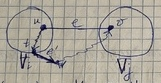
\includegraphics[width=0.45\textwidth]{./images/1.jpg}
%   \end{center}
% \end{figure}
% }
%
% \begin{algorithm}
%   \caption{Крускала}
%   \begin{algorithmic}[1]
%     \Require{$Qs$ --- очередь с ??? для рёбер}
%     \Ensure{$Vs$ --- набор непересекающихся подмножеств вершин}
%     \State{$T$ = $\emptyset$, $Vs$ = $\emptyset$}
%     \State{Создаём очередь с ??? $Q$ из всех рёбер из $E$}
%     \ForAll{$v$ $\in$ $V$}
%       \State{Добавить \{$v$\} к $Vs$}
%     \EndFor
%     \While{|$Vs$|>1}
%       \State{($v$,$w$)= MIN($Q$); УДАЛИТЬ($Q$,($v$,$w$))}
%       \State{$w_1$ = НАЙТИ($v$); $w_2$ = НАЙТИ($w$)}
%       \If{$w_1\neq w_2$}
%         \State{ОБЪЕДИНИТЬ($w_1,w_2,w_1$)}
%         \State{$T$ = $T$ $\cup$ \{($v$,$w$)\}}
%       \EndIf
%     \EndWhile
%   \end{algorithmic}
% \end{algorithm}
%
% \thm{}{Алгоритм Крускала строит минимальное остовное дерево для связного
% неориентированного графа $G=(V,E)$.\\ Если в цикле в строках 4-11
% рассматривается $d$ рёбер, то \textbf{время работы} составляет
% $O(d\log\limits_2|E| + |E|\log\limits_2|E|) \leq
% O(|E|\log\limits_2|E|)$}
\chapter{}
\section{Потоки в сетях}
\dfn{Сеть}{
  Пятёрка $N=(V,E,s,t,c)$, где:\\
  $(V,E)$ --- ориентированный граф\\
  $s\in V$ --- источник, вершина, в которую не входят рёбра\\
  $t\in V$ --- сток, вершина, из которой не выходят рёбра\\
  $c: E\rightarrow R_+$ --- прорускные способности рёбер.
}

\dfn{Поток в сети f}{
  Отображение f: E$\rightarrow$R такое, что:
  \begin{enumerate}
    \item $0\leq f(e)\leq c(e)$ для всех $e\in E$;
    \item $\displaystyle\sum\{f(u,v): (u,v)\in E\} = \displaystyle\sum\{f(v,u):(v,u)\in E\}$ для $v\notin\{s,t\}$
  \end{enumerate}
  (2) --- закон Кирхгофа: величина потока f: $val(f)=\displaystyle\sum_{(s,v)\in E}f(s,v)$
}

\dfn{Максимальный поток}{
  Поток с наибольшей величиной.
}

\newpage
\ex{Пример графа потоков в сетях}{
  Обозначения: 
  \begin{itemize}
    \item число в скобках --- пропускная способность,
    \item число без скобок --- величина потока по ребру(поток по ребру).
  \end{itemize}
  % рисунок 1
  \begin{figure}[H]
    \begin{center}
      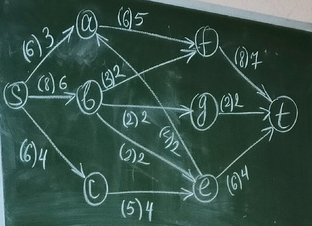
\includegraphics[width=0.45\textwidth]{./images/2.jpg}
    \end{center}
  \end{figure}

  $val(f)=3+6+4 = 13$ --- не максимальный поток.
}

\dfn{Разрез в сети $N=(V,E,s,t,c)$}{
  Множество $A\subseteq V$ такое, что $s \in A, t\notin A.$\\
  Любое множество вершин, содержащее источник, но не содержащее сток.
}

\dfn{P(A)}{
  $A\subseteq V$(Не обязательно разрез)\\
  P(A) = $\{(u,v):u\in A,v\in V\backslash A\}$ --- все рёбра, выходящие из множества A наружу.
}

\dfn{Пропускная способность разреза A}{
  %\ вместо /
  $c(A,V\backslash A) = \displaystyle\sum_{(u,v)\in P(A)} c(u,v)$
}

\dfn{Минимальный разрез}{
  Разрез с минимальной пропускной способностью.
}

\dfn{Поток через разрез A}{
  %\ вместо /
  $f(A,V\backslash A) = \displaystyle\sum_{(u,v)\in P(A)} f(u,v)$
}

\ex{}{
  $A = \{s,a,b\}$\\
  $P(A)=\{(a,f),(b,e),(b,f),(b,g),(s,c)\}$\\
  $P(V/A)=\{(e,a)\}$\\
  $c(A,V\backslash A)=6+2+3+2+6=19$\\
  $f(A,V\backslash A)=5+2+2+2+4=15$\\
  $f(V\backslash A,A)=2$\\
  $f(A,V\backslash A)-f(V\backslash A,A)=15-2=13$
}
\ex{}{
  $B = \{s,e,f\}$\\
  $P(B)=\{(s,a),(s,b),(s,c),(e,a),(e,t),(f,t)\}$\\
  $P(V/B)=\{(b,e),(c,e),(a,f),(b,f)\}$\\
  $c(B,V\backslash B)=6+8+6+4+6+8=38$\\
  $f(B,V\backslash B)=3+6+4+2+4+7=26$\\
  $f(V\backslash B,B)=2+4+5+2=13$\\
  $f(B,V\backslash B)-f(V\backslash B,B)=26-13=13$
}

\mprop{}{
  Если $(u,v)\notin E$, то $c(u,v)=0,f(u,v)=0$
}

\mlenma{}{
  $val(f)=f(A,V\backslash A)-f(V\backslash A,A)$ для любого потока или разреза A.
}

\pf{Доказательство}{
  $\displaystyle\sum_{v\in V}f(u,v) - \displaystyle\sum_{v\in V}f(v,u) = \begin{cases}
    val(f), \text{ если } u = s,\\
    0, \text{ если } u = s,
  \end{cases}\\
  \displaystyle\sum_{u\in A}\displaystyle\sum_{v\in V}f(u,v)-\displaystyle\sum_{u\in A}\displaystyle\sum_{v\in V}f(v,u)=val(f)\\
  u\in A,v\in A$ --- слагаемые взаимно уничтожаются.\\
  Тогда:\\
  $\displaystyle\sum_{u\in A}\displaystyle\sum_{v\in V\backslash A}f(u,v)-\displaystyle\sum_{u\in A}\displaystyle\sum_{v\in V\backslash A}f(v,u)=val(f)\\$
  $f(A,V\backslash A)-f(V\backslash A,A)=val(f)$
}

\cor{}{
  $val(f)= \displaystyle\sum_{v\in V}f(v,t)$
}

\thm{Форд, Фалкерсон}{
  Величина любого потока в сети не превосходит пропускной способности минимального разреза.
}
\pf{Доказательство}{
  $A$ --- разрез($s\in A,t\notin A$)\\
  $val(f) = f(A,V\backslash A)-f(V\backslash A,A)\leq f(A,V\backslash A)=\displaystyle\sum_{e\in P(A)}f(e)\leq\displaystyle\sum_{e\in P(A)}c(e)=c(A,V\backslash A)$
}

\dfn{Увеличивающий путь относительно потока $f$ из $s$ в $v$}{
  Последовательность вершин $\mvec{v}{n}$ такая, что:
  \begin{enumerate}
    \item $v_0=s,v_n=v$
    \item $(v_i,v_{i+1})\in E$ или $(v_{i+1},v_{i})\in E$
    \item если $(v_i,v_{i+1})\in E$, то $f(v_i,v_{i+1})<c(v_i,v_{i+1})$
    \item если $(v_{i+1},v_i)\in E$, то $f(v_{i+1},v_i)>0$
  \end{enumerate}
  Ребро $e$ насыщенное, если $f(e)=c(e)$.\\
  Ребро $e$ непустое, если $f(e)>0$.
}

\ex{Примеры увеличивающих путей} {
  В графе из примера 1 увеличивающими являются пути:\\
  $s\xrightarrow{(6)3}a\xrightarrow{(6)5}f\xrightarrow{(8)7}t$,\\
  $s\xrightarrow{(6)3}a\xleftarrow{(4)2}e\xrightarrow{(6)4}t$.\\
  В то время как путь
  $s\xrightarrow{(8)6}b\xrightarrow{(2)2}g\xrightarrow{(2)2}t$ увеличивающим не является.
}

\thm{}{
  Следующие условия эквивалентны:
  \begin{enumerate}
    \item поток $f$ максимальный
    \item не существует увеличивающего пути относительно $f$
    \item для некоторого разреза $A val(f)=c(A,V\backslash A).$
  \end{enumerate}
}
\pf{Доказательство}{
  1)$\Rightarrow$2) От противного.\\
  $(s=v_0,v_1,\dots,v_{k-1},v_k=t)$ --- увеличивающий путь.\\
  $e_i=(v_i,v_{i+1})\\
  \Delta(e_i)=\begin{cases}
    c(e_i)-f(e_i), \text{ если } e_i \text{ ---  прямое ребро}\\
    f(e_i), \text{ если } e_i \text{ ---  обратное ребро}\\
  \end{cases}$\\
  $\Delta(e_i)>0\\
  \delta=min\{\Delta(e_i):0\leq i\leq k-1\}$\\
  $\delta>0\\
  f' \text{ --- новый поток}\\
  f'(e)=\begin{cases}
    f(e)+\delta, \text{ если e --- прямое ребро}\\
    f(e)-\delta, \text{ если e --- обратное ребро}\\
    f(e), \text{иначе}
  \end{cases}$
  % картинка со стрелочками
  \begin{figure}[H]
    \begin{center}
      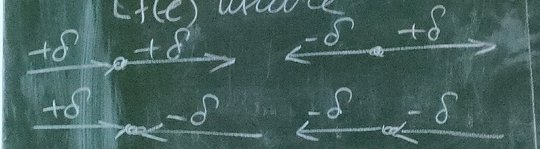
\includegraphics[width=0.45\textwidth]{./images/3.jpg}
    \end{center}
  \end{figure}
  $val(f')=val(f)+\delta\\
  f$ --- не максимальный. Противоречие.

  2)$\Rightarrow$3)\\
  $A=\{v\in V:\text{ существует увеличивающий путь из $s$ в $v$}\}$\\
  $A$ --- разрез, так как $t\notin A$(по условию)\\
  % рисунок
  $(u,v)$ --- прямое ребро $\Rightarrow f(u,v)=c(u,v)$\\
  $(u,v)$ --- обратное ребро $\Rightarrow f(u,v)=0$\\
  Иначе можно продлить увеличивающий путь\\
  $var(f) = f(A,V\backslash A)-f(V\backslash A,A) = \displaystyle\sum_{e\in P(A)}f(e)-\displaystyle\sum_{e\in P(V\backslash A)}f(e)=\\=\displaystyle\sum_{e\in P(A)}c(e)=c(A,V\backslash A)$

  3)$\Rightarrow$1) По теореме 1.
}

\thm{Форд, Фалкерсон}{
  Величина максимального потока равна пропускной способности минимального разреза.
}
\pf{Доказательство}{
  $A$ --- минимальный разрез\\
  $f$ --- максимальный поток\\
  $val(f) \leq c(A,V\backslash A)$ --- по теореме 1\\
  Если $val(f) < c(A,V\backslash A)$, то $f$ не максимальный по теоремме 2.\\
  Следовательно, $val(f) = c(A,V\backslash A)$
}

\mprop{Структуры данных в алгоритме Форда-Фолкенсона}{
\begin{itemize}
  \item $L(v)$ --- предшественник $v$ в увеличивающем пути.
  \item $\delta(v)$ --- величина дополнительного потока из $s$ в $v$.
  \item $Q$ --- очередь вершин.
  \item Вершины пронумерованы числами 1,2,\dots
\end{itemize}
}

\malg{ПРОСМОТРЕТЬ}{v}{ничего}{
  \ForAll{$(v,u)\in E$}
    \If{$L(u)=0$ и $f(v,u)<c(v,u)$}
      \State $L(u) = v;$
      \State $\delta(u)=min\{\delta(v),c(v,u)-f(v,u)\};$
      \State ДОБАВИТЬ($Q,u$);
    \EndIf
  \EndFor
  \ForAll{$(v,u)\in E$}
    \If{$L(u)=0$ и $f(u,v)>0$}
      \State $L(u)=-v;$
      \State $\delta(u)=min\{\delta(u),f(u,v)\};$
      \State ДОБАВИТЬ($Q,u$);
    \EndIf
  \EndFor
}
\malg{Форда-Фолкерсона}{сеть $N=(V,E,s,t,c)$}{максимальный поток $f$ в $N$}{
  \State готово = "нет"
  \ForAll{$e\in E$}
    \State $f(e) = 0$;
  \EndFor
  \While{готово = "нет"}
    \ForAll{$v\in V\backslash \{s\}$}
      \State $L(v)=0; \delta(v) = 0;$
    \EndFor
    \State $L(s) = s;\delta(s)=\infty;$
    \State Добавить(Q,s);
    \While{$Q\neq\emptyset$}
      \State $v=$НАЧАЛО($Q$);
      \State УДАЛИТЬ($Q,v$);
      \State ПРОСМОТРЕТЬ($v$);
    \EndWhile
    \If{$L(t)\neq 0$}
      \State $v=t$;
      \While{$v\neq s$}
        \State $u=L(v);$
        \If{$u>0$}
          \State $f(u,v)=f(u,v)+\delta(t);$
        \Else 
          \State $f(v,u)=f(v,u)-\delta(t);$
        \EndIf
        \State $v=|u|$
      \EndWhile
    \Else
      \State готово = "да";
    \EndIf
  \EndWhile
}

\newpage
\ex{Пример применения алгоритма Форда-Фолкерсона}{
  Применить алгоритм к сети из примера 1.\\
  Шаги алгоритма:
  \begin{figure}[H]
    \begin{center}
      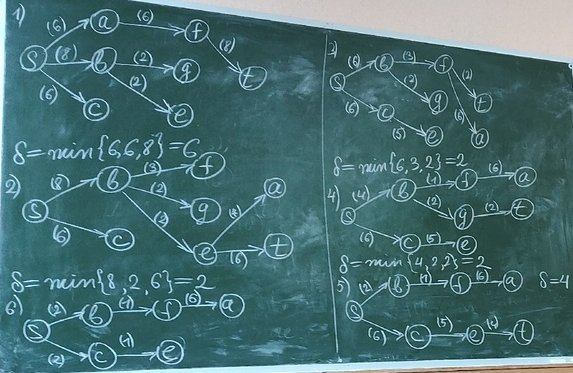
\includegraphics[width=0.9\textwidth]{./images/4.jpg}
    \end{center}
  \end{figure}
  Итоговый граф потоков:
  \begin{figure}[H]
    \begin{center}
      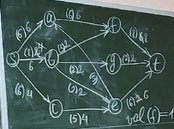
\includegraphics[width=0.45\textwidth]{./images/5.jpg}
    \end{center}
  \end{figure}
}

\newpage
\qs{Применить алгоритм Форда-Фолкерсона}{
  Исходный граф(после зачёркиваний новые значения, получаемые на шагах алгоритма):
  \begin{figure}[H]
    \begin{center}
      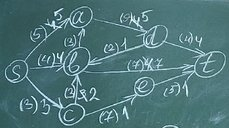
\includegraphics[width=0.45\textwidth]{./images/6.jpg}
    \end{center}
  \end{figure}
  Шаги алгоритма:
  \begin{figure}[H]
    \begin{center}
      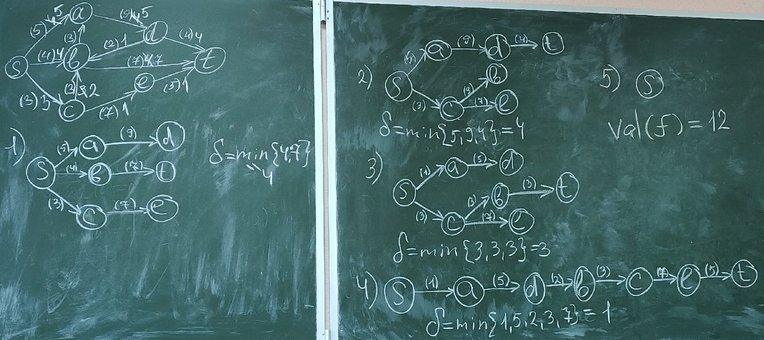
\includegraphics[width=0.9\textwidth]{./images/7.jpg}
    \end{center}
  \end{figure}
}

\end{document}
